% Länge 1: 32,5 cm
% Länge 2: 65,3 cm
% normale Schwingung:
% Exp L1:   T_linkes_L1: 1,237+/-0,005 in s         T_rechtes_L1: 1,238+/-0,004in s
% Exp L2 :  T_linkes_L2: 1,602+/-0,006 in s         T_rechtes_L2: 1,608+/-0,006in s
% gleichsinnige Schwingung:
% Exp L1:   T_gleich_L1: 1,194+/-0,004 in s         omega_gleich_L1: 5,261+/-0,017 in 1/s
% Theo L1:  T_plus_1_theo: 1,1436339652282395 in s  omega_plus_1_theo: 5,494052728598024 in 1/s
% Exp L2:   T_gleich_L2: 1,567+/-0,010 in s         omega_gleich_L2: 4,009+/-0,025 in 1/s
% Theo L2:  T_plus_2_theo: 1,6210706966168085 in s  omega_plus_2_theo: 3,875947742620146 in 1/s
% gegensinnige Schwingung
% Exp L1:   T_gegen_L1: 1,031+/-0,008 in s          omega_gegen_L1: 6,09+/-0,05 in 1/s
% Theo L1:  T_mius_1_theo: 0,988+/-0,008 in s       omega_minus_1_theo: 6,36+/-0,05 in 1/s
% Exp L2:   T_gegen_L2: 1,420+/-0,006 in s          omega_gegen_L2: 4,426+/-0,017 in 1/s
% Theo L2:  T_mius_2_theo: 1,468+/-0.011 in s       omega_minus_2_theo: 4,279+/-0,031 in 1/s
% Kopplungskonstanten:  
% Kopplungskonstante K_L1:    0,146+/-0,008 
% Kopplungskonstante K_L2:    0,099+/-0,007 
% Gekoppelte Schwingung 
% Exp L1:   T_schwingung_L1: 1,10+/-0,04 in s       Exp?????: omega_schwingung_L1: 5,72+/-0,20 in 1/s
% Exp L1:   T_schwebung_L1: 7,119+/-0,009 in s      omega_schwebung_L1: -0,83+/-0,05 in 1/s bzw. 0,8826+/-0,0011 in 1/s (2*pi*(1/T))
% Theo L1:  T_schwebung_L1_theo: 7,2+/-0,4 in s     omega_schwebung_L1_theo: -0,87+/-0,05 in 1/s
% Exp L2:   T_schwingung_L2: 1,546+/-0,011 in s     Exp?????: omega_schwingung_L2: 4,065+/-0,030 in 1/s
% Exp L2:   T_schwebung_L2: 15,741+/-0,013 in s     omega_schwebung_L2: -0,417+/-0.030 in 1/s bzw. 0,39917+/-0,00033 in 1/s (2*pi*(1/T))
% Theo L2:  T_schwebung_L2_theo: 15,6+/-1,2 in s    omega_schwebung_L2_theo: -0,404+/-0,031 in 1/s
\section{Auswertung}
\label{sec:Auswertung}
\nocite{anleitungV106}
%
\subsection{Kurzes Pendel}
\label{sec:Auswertung_KuresPendel}
Zunächst werden die beiden Schwingungen der einzelnen Pendel bei einer Länge von $32,5\, \unit{\centi\meter}$ verglichen. Die gemessene fünffache Schwingungsdauer $5\,T$ des linken als auch des rechten
Pendels sind in der Tabelle (\ref{tab:EinzelSchwingung_L1}) aufgelistet.
\begin{table}[H]
  \centering
  \caption{Gemessene fünffache Schwingungsdauer bei einer Länge von $32,5\, \unit{\centi\meter}$.}
  \label{tab:EinzelSchwingung_L1}
  \begin{tblr}{colspec={c c}}
      \toprule
      linkes Pendel & rechtes Pendel\\ 
      $5\, T_{\text{l}, 1}\,\left[\unit{\second}\right]$ & $5\, T_{\text{r}, 1}\,\left[\unit{\second}\right]$  \\
      \midrule
      6,21 & 6,19 \\
      6,07 & 6,24 \\
      6,15 & 6,24 \\
      6,19 & 6,30 \\
      6,24 & 6,05 \\
      6,10 & 6,15 \\
      6,22 & 6,18 \\
      6,14 & 6,18 \\
      6,19 & 6,14 \\
      6,35 & 6,25 \\
      \bottomrule
  \end{tblr}
\end{table}
Aus dieser Tabelle und mit den Gleichungen $$\bar{x} = \frac{1}{n} \cdot \sum_{i = 1}^{n}x_i$$ und $$\Delta \bar{x} = \sqrt{\frac{1}{n \cdot (n - 1)} \cdot \sum_{i = 1}^{n}(x_i - \bar{x})} $$
lassen sich die Mittelwerte sowie die Standardabweichung des Mittelwerts bestimmen. $x_i$ beschreibt die einzelnen Messdaten und $n$ die Anzahl
der Messungen. Somit ergeben sich die Schwingungsdauern und deren Standardabweichungen
\begin{align*}
  T_{\text{l,exp.}, 1} &= \left( 1,237 \pm 0,005 \right)\,\unit{\second}\\
  T_{\text{r,exp.}, 1} &= \left( 1,238 \pm 0,004 \right)\,\unit{\second}\,.
\end{align*}
Aufgrund der Fehlertolernz werden die beiden Pendel als identisch angenommen. Daher wird im Folgenden mit der Untersuchung der drei verschiedene Schwingungsarten
begonnen.
%
%
\subsubsection{Gleichphasige Schwingung}
\label{sec:GleichphasigeSchwingung_KuresPendel}
Die gemessene fünffache Schwingungsdauer der gleichphasigen Schwingung sind in der Tabelle (\ref{tab:GleichphasigeSchwingung_L1}) aufgeführt.
\begin{table}[H]
  \centering
  \caption{Gemessene fünffache Schwingungsdauer bei einer Länge von $32,5\, \unit{\centi\meter}$ und gleichphasiger Schwingung.}
  \label{tab:GleichphasigeSchwingung_L1}
  \begin{tblr}{colspec={c}}
      \toprule
      $5\, T_{+, 1}\,\left[\unit{\second}\right]$\\
      \midrule
      5,97 \\
      5,88 \\
      5,92 \\
      5,98 \\
      5,97 \\
      5,99 \\
      5,95 \\
      6,02 \\
      6,10 \\
      5,93 \\
      \bottomrule
  \end{tblr}
\end{table}
Die aus der Tabelle (\ref{tab:GleichphasigeSchwingung_L1}) hergeleitete, gemittelte Schwingungsdauer mit der Standardabweichung lautet
$$T_{+,\text{exp.}, 1} = \left( 1,194 \pm 0,004 \right)\,\unit{\second}\,.$$
Durch Einsetzen von Gleichung (\ref{eqn:OmegaGleichsinnig}) in die Gleichung (\ref{eqn:VerbindungTOmega}) wird die theoretische Schwingungsdauer der gleichphasigen Schwingung bestimmt. Daraus folgt
$$T_{+, \text{theo.}, 1} = 1,144\,\unit{\second}\,.$$
Aus der Gleichung (\ref{eqn:VerbindungOmegaT}) und der Gaußschen Fehlerfortpflanzung 
$$\Delta \omega = \sqrt{\left(-\frac{2 \pi}{T^{2}}\cdot \Delta T \right)^{2}}$$
wird, durch Einsetzen von $T_{\text{gl}, 1}$, die Schwingungsfrequenz
$$\omega_{+,\text{exp.}, 1} =  \left( 5,261 \pm 0,017 \right)\,\unit[per-mode=fraction]{\per \second}$$ berechnet. 
Anhand der Gleichung (\ref{eqn:OmegaGleichsinnig}) wird die theoretische Schwingungsfrequenz der gleichphasigen Schwingung 
$$\omega_{+, \text{theo.}, 1} = 5,494\,\unit[per-mode=fraction]{\per \second}\,$$ bestimmt.
%
%
\subsubsection{Gegenphasige Schwingung}
\label{sec:GegenphasigeSchwingung_KurzelPendel}
Die gemessenen Schwingungsdauern der gegenphasigen Schwingung bei einer Länge von $32,5\, \unit{\centi\meter}$ sind 
in der Tabelle (\ref{tab:GegenphasigeSchwingung_L1}) aufgeführt. 
\begin{table}[H]
  \centering
  \caption{Gemessene fünffache Schwingungsdauer bei einer Länge von $32,5\, \unit{\centi\meter}$ und gegenphasiger Schwingung.}
  \label{tab:GegenphasigeSchwingung_L1}
  \begin{tblr}{colspec={c}}
      \toprule
      $5\, T_{-, 1}\,\left[\unit{\second}\right]$\\
      \midrule
      5,10 \\
      5,20 \\
      5,13 \\
      5,45 \\
      5,08 \\
      5,06 \\
      5,08 \\
      5,06 \\
      5,30 \\
      5,10 \\
      \bottomrule
  \end{tblr}
\end{table}
Anhand dieser Daten lassen sich die gemittelte Schwingungsdauer und die Standardabweichung berechnen. Somit ergibt sich
$$T_{-,\text{exp.}, 1} = \left(1,031 \pm 0,008 \right)\, \unit{\second}\,.$$ 
Für die Bestimmung der theoretischen Schwingungsdauer und Schwingungsfrequenz einer gegenphasigen Schwingung wird die Kopplungskonstante $K$ benötigt. Da
diese nicht gegeben ist, wird die Kopplungskonstante durch Einsetzen von $T_{+,1}$ und $T_{-,1}$ in die Gleichung (\ref{eqn:Kopplungskonstante}) berechnet. Die Messunsicherheit der Kopplungskonstante
ergibt sich aus der Gaußschen Fehlerfortpflanzung
$$\Delta K = \sqrt{\left(\frac{4 \cdot T_+\cdot T_{-}^{2}}{\left(T_{+}^{2} + T_{-}^{2}\right)^{2}}\cdot \Delta T_+\right)^{2}+ \left(-\frac{4\cdot T_{+}^{2}\cdot T_{-}}{\left(T_{+}^{2} + T_{-}^{2}\right)^{2}} \cdot \Delta T_{-}\right)^2}\,.$$
Daraus folgt
$$K_1 = \left( 0,146 \pm 0,008 \right)\,.$$
Anschließend lässt sich die theoretische Schwingungsdauer mithilfe der Gleichungen (\ref{eqn:VerbindungTOmega}) und (\ref{eqn:OmegaGegensinnig}) bestimmen. Diese lautet
$$T_{-,\text{theo.},1} = \left( 0,988 \pm 0,008 \right)\, \unit{\second}\,.$$
Die empirische Schwingungsfrequenz 
$$\omega_{-,\text{exp.},1} = \left( 6,09 \pm 0,05 \right)\, \unit[per-mode=fraction]{\per \second}$$ wird durch $T_{-,1}$ und der Gleichung (\ref{eqn:VerbindungOmegaT})
berechnet. Aus der Gleichung (\ref{eqn:OmegaGegensinnig}) ergibt sich die folgendene theoretische Schwingungsfrequenz
$$\omega_{-,\text{theo.},1} = \left( 6,36 \pm 0,05 \right)\,\unit[per-mode=fraction]{\per \second}\,.$$
%
%
\subsubsection{Gekoppelte Schwingung}
\label{sec:GekoppelteSchwingung_KurzesPendel}
In der Tabelle (\ref{tab:Gekoppelt_L1}) sind die Schwingungsdauer und die Schwebung einer gekoppelten Schwingungen aufgelistet.
\begin{table}[H]
  \centering
  \caption{Gemessene fünffache Schwingungsdauer und Schwebung bei einer Länge von $32,5\, \unit{\centi\meter}$ und gekoppelter Schwingung.}
  \label{tab:Gekoppelt_L1}
  \begin{tblr}{colspec={c c}}
      \toprule
      $5\, T_{1}\,\left[\unit{\second}\right]$ & $5\, T_{\text{S}, 1}\,\left[\unit{\second}\right]$  \\
      \midrule
      5,09 & 35,53 \\
      4,93 & 35,94 \\
      4,76 & 35,56 \\
      5,03 & 35,58 \\
      5,56 & 35,63 \\
      5,20 & 35,58 \\
      5,69 & 35,50 \\
      5,70 & 35,44 \\
      6,50 & 35,55 \\
      6,46 & 35,64 \\
      \bottomrule
  \end{tblr}
\end{table}
Aus dieser Tabelle lassen sich die gemittelte Schwingungsdauer und die Standardabweichung 
$$T_{1,\text{exp.}} = \left( 1,10\pm 0,04 \right)\, \unit{\second}$$ bestimmen.
Durch Einsetzen der Schwingungsdauer $T_{1,\text{exp.}}$ in die Gleichung (\ref{eqn:VerbindungOmegaT}) ergibt sich die Schwingungsfrequenz
$$\omega_{1,\text{exp.}} = \left( 5,72 \pm 0,20 \right)\, \unit[per-mode=fraction]{\per \second}\,.$$
Anhand der Messwerte aus der Tabelle (\ref{tab:Gekoppelt_L1}) werden die gemittelte Schwebung und die Standardabweichung 
$$T_{\text{S,exp.},1} = \left( 7,119 \pm 0,009 \right)\, \unit{\second}$$ berechnet. 
Der theoretische Wert berechnet sich mit der Gleichung (\ref{eqn:TSchwebung}) und beträgt
$$T_{\text{S,theo.},1} = \left( 7,2 \pm 0,4 \right)\, \unit{\second}\,.$$
Die aus der Gleichung (\ref{eqn:VerbindungOmegaT}) ermittelte Schwingungsfrequenz der Schwebung, durch Einsetzen von $T_{\text{S,exp.},1}$, lautet
$$\omega_{\text{S,exp.},1} = \left( 0,8826 \pm 0,0011 \right)\unit[per-mode=fraction]{\per \second}\,.$$
Mithilfe der Gleichung (\ref{eqn:OmegaSchwebung}) wird die theoretische Schwingungsfrequenz berechnet. Der Betrag davon lautet
$$\omega_{\text{S,theo.},1} = \left( 0,87 \pm 0,05 \right)\unit[per-mode=fraction]{\per \second}\,.$$
%
%
\subsection{Langes Pendel}
\label{sec:Auswertung_LangesPendel}
Zunächst werden erneut die beiden einzelnen Schwingungen bei einer Länge von $65,3\, \unit{\centi\meter}$ miteinander verglichen. Die dafür gemessenen Schwingungsdauern sind in der Tabelle (\ref{tab:EinzelSchwingung_L2})
aufgeführt.
\begin{table}[H]
  \centering
  \caption{Gemessene fünffache Schwingungsdauer bei einer Länge von $65,3\, \unit{\centi\meter}$.}
  \label{tab:EinzelSchwingung_L2}
  \begin{tblr}{colspec={c c}}
      \toprule
      linkes Pendel & rechtes Pendel\\ 
      $5\, T_{\text{l}, 2}\,\left[\unit{\second}\right]$ & $5\, T_{\text{r}, 2}\,\left[\unit{\second}\right]$  \\
      \midrule
      7,99 & 7,96 \\
      8,04 & 7,96 \\
      7,96 & 8,11 \\
      7,99 & 7,97 \\
      8,04 & 7,96 \\
      8,17 & 8,04 \\
      7,92 & 8,14 \\
      7,94 & 8,16 \\
      7,89 & 7,97 \\
      8,18 & 8,14 \\
      \bottomrule
  \end{tblr}
\end{table}
Aus der Tabelle ergeben sich die gemittelten Schwingungsdauern und deren Standardabweichungen
\begin{align*}
  T_{\text{l,exp.}, 2} &= \left( 1,602 \pm 0,006 \right)\, \unit{\second}\\
  T_{\text{r,exp.}, 2} &= \left( 1,608 \pm 0,006 \right)\, \unit{\second}\,.
\end{align*}
Aufgrund der Fehlertoleranz werden die beiden Pendel erneut als identisch angenommen und die drei verschiedene Schwingungsarten untersucht.
\subsubsection{Gleichphasige Schwingung}
\label{sec:GleichphasigeSchwingung_LangesPendel}
Die gemessenen Schwingungsdauern einer gleichphasigen Schwingung bei einer Länge von $65,3\, \unit{\centi\meter}$ sind in der Tabelle (\ref{tab:GleichphasigeSchwingung_L2})
aufgelistet. 
\begin{table}[H]
  \centering
  \caption{Gemessene fünffache Schwingungsdauer bei einer Länge von $65,3\, \unit{\centi\meter}$ und gleichphasiger Schwingung.}
  \label{tab:GleichphasigeSchwingung_L2}
  \begin{tblr}{colspec={c}}
      \toprule
      $5\, T_{+, 2}\,\left[\unit{\second}\right]$\\
      \midrule
      7,82 \\
      8,09 \\
      7,70 \\
      8,06 \\
      7,83 \\
      7,95 \\
      7,65 \\
      7,72 \\
      7,72 \\
      7,83 \\
      \bottomrule
  \end{tblr}
\end{table}
Aus diesen Werten ergeben sich die gemittelte Schwingungsdauer und die Standardabweichung
$$T_{+,\text{exp.},2} = \left( 1,567 \pm 0,010 \right)\, \unit{\second}\,.$$
Die theoretische Schwingungsdauer lässt sich anhand der Gleichungen (\ref{eqn:VerbindungTOmega}) und (\ref{eqn:OmegaGleichsinnig}) bestimmen und beträgt
$$T_{+,\text{theo.},2} = 1,621\, \unit{\second}\,.$$
Mit der Gleichung (\ref{eqn:VerbindungOmegaT}) und $T_{+,\text{exp.},2}$ lässt sich die Schwingungsfrequenz
$$\omega_{+,\text{exp.},2} = \left( 4,009 \pm 0,025 \right)\, \unit[per-mode=fraction]{\per\second}$$ berechnen. 
Die theoretische Schwingungsfrequenz
$$\omega_{+,\text{theo.},2} = 3,876 \, \unit[per-mode=fraction]{\per\second}$$ ergibt sich aus der Gleichung (\ref{eqn:OmegaGleichsinnig}).

%
%
\subsubsection{Gegenphasige Schwingung}
\label{sec:GegenphasigeSchwingung_LangesPendel}
In der Tabelle (\ref{tab:GegenphasigeSchwingung_L2}) sind die gemessenen Schwingungsdauern bei einer Länge von $65,3\, \unit{\centi\meter}$ einer gegenphasigen
Schwingung. 
\begin{table}[H]
  \centering
  \caption{Gemessene fünffache Schwingungsdauer bei einer Länge von $65,3\, \unit{\centi\meter}$ und gegenphasiger Schwingung.}
  \label{tab:GegenphasigeSchwingung_L2}
  \begin{tblr}{colspec={c}}
      \toprule
      $5\, T_{-, 2}\,\left[\unit{\second}\right]$\\
      \midrule
      7,18 \\
      7,09 \\
      7,04 \\
      7,01 \\
      7,24 \\
      7,13 \\
      7,06 \\
      7,10 \\
      7,18 \\
      6,95 \\
      \bottomrule
  \end{tblr}
\end{table}
Aus dieser Tabelle ergeben sich die gemittelte Schwingungsdauer und die Standardabweichung
$$T_{-,\text{exp.},2} = \left(1,420 \pm 0,006\right)\,\unit{\second}\,.$$
Um die theoretische Schwingungsdauer zu bestimmt wird zunächst die Kopplungskonstante $K$ mit der
Gleichung (\ref{eqn:Kopplungskonstante}) bestimmt. Daraus ergibt sich
$$K_{2} = 0,099 \pm 0,007\,.$$
Durch Einsetzen von Gleichung (\ref{eqn:OmegaGegensinnig}) in die Gleichung (\ref{eqn:VerbindungTOmega}) wird die theoretische Schwingungsdauer 
$$T_{-,\text{theo.},2} = \left( 1,468 \pm 0.011 \right)\,\unit{\second}$$ berechnet. Durch Einsetzen von
$T_{-,\text{exp.},2}$ in die Gleichung (\ref{eqn:VerbindungOmegaT}) wird die Schwingungsfrequenz 
$$\omega_{-,\text{exp.},2} = \left(4,426 \pm 0,017 \right)\, \unit[per-mode=fraction]{\per\second}$$ bestimmt. 
Für die theoretische Schwingungsfrequenz ergibt sich aus der Gleichung (\ref{eqn:OmegaGegensinnig}) 
$$\omega_{-,\text{theo.},2} = \left( 4,279 \pm 0,031 \right)\, \unit[per-mode=fraction]{\per\second}\,.$$
%
%
\subsubsection{Gekoppelte Schwingung}
\label{sec:GekoppelteSchwingung_LangesPendel}
Die gemessenen Schwingungsdauern bei der gekoppelten Schwingung sind in der Tabelle (\ref{tab:Gekoppelt_L2}) aufgeführt.
\begin{table}[H]
  \centering
  \caption{Gemessene fünffache Schwingungsdauer und Schwebung bei einer Länge von $65,3\, \unit{\centi\meter}$ und gekoppelter Schwingung.}
  \label{tab:Gekoppelt_L2}
  \begin{tblr}{colspec={c c}}
      \toprule
      $5\, T_{2}\,\left[\unit{\second}\right]$ & $5\, T_{\text{S}, 2}\,\left[\unit{\second}\right]$  \\
      \midrule
      7,63 & 78,36 \\
      7,89 & 78,86 \\
      7,73 & 78,50 \\
      8,16 & 78,82 \\
      7,60 & 78,46 \\
      7,60 & 78,89 \\
      7,60 & 78,58 \\
      7,61 & 78,81 \\
      7,69 & 78,93 \\
      7,78 & 78,82 \\
      \bottomrule
  \end{tblr}
\end{table}
Aus diesen Messwerten lässt sich die gemittelte Schwingungsdauer mit der Standardabweichung
$$ T_{2,\text{exp.}} =\left( 1,546 \pm 0,011 \right)\,\unit{\second} $$ ermitteln. 
Die Schwingungsfrequenz wird aus der Gleichung (\ref{eqn:VerbindungOmegaT}) berechnet. Daraus folgt
$$\omega_{2,\text{exp.}} = \left( 4,065 \pm 0,030 \right)\, \unit[per-mode=fraction]{\per\second}\,.$$
Die gemittelte Schwebung mit der Standardabweichung wird anhand der Messwerte aus der Tabelle (\ref{tab:Gekoppelt_L2}) berechnet.
Somit ergibt sich
$$T_{\text{S,exp.},2} = \left( 15,741 \pm 0,013 \right)\,\unit{\second}\,.$$
Mithilfe der Gleichung (\ref{eqn:TSchwebung}) wird die folgende theoretische Schwebung bestimmt
$$ T_{\text{S,theo.},2} = \left( 15,6 \pm 1,2 \right)\,\unit{\second}\,.$$
Durch Einsetzen von $T_{\text{S,exp.},2}$ in Gleichung (\ref{eqn:VerbindungOmegaT}) wird die Schwebungsfrequenz
$$\omega_{\text{S,exp.},2} = \left( 0,39917 \pm 0,00033  \right)\, \unit[per-mode=fraction]{\per\second} $$ berechnet.
Anhand der Gleichung (\ref{eqn:OmegaSchwebung}) lässt sich die theoretische Schwebungsfrequenz ermitteln. Der Betrag davon lautet
$$\omega_{\text{S,theo.},2} = \left( 0,404 \pm 0,031  \right)\, \unit[per-mode=fraction]{\per\second}\,.$$ 
% \begin{figure}
%   \centering
%   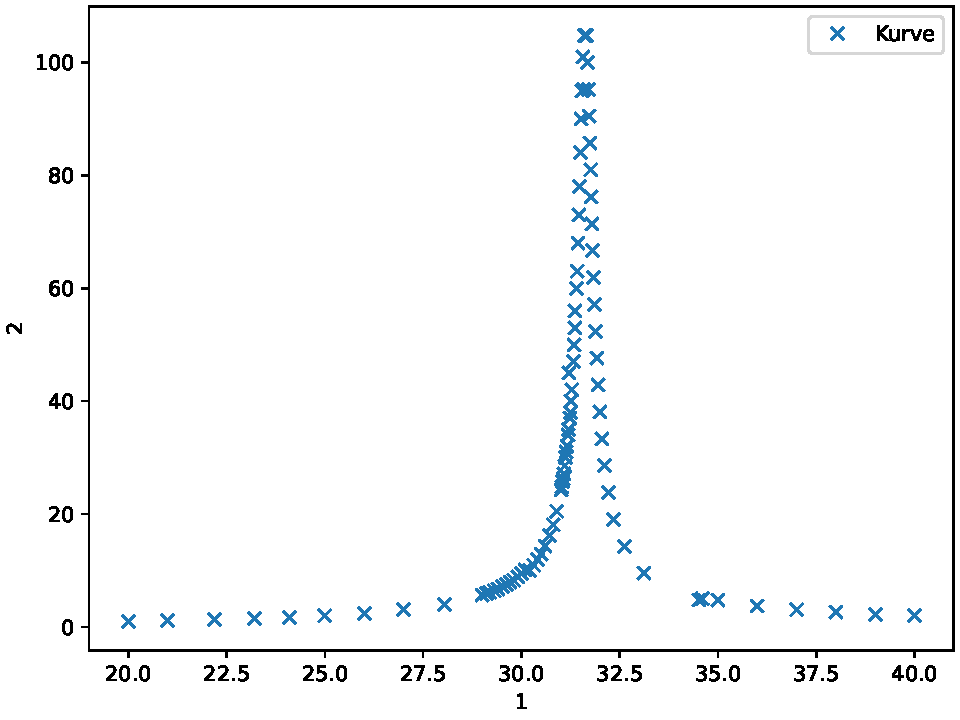
\includegraphics{plot.pdf}
%   \caption{Plot.}
%   \label{fig:plot}
% \end{figure}

%Siehe \autoref{fig:plot}!